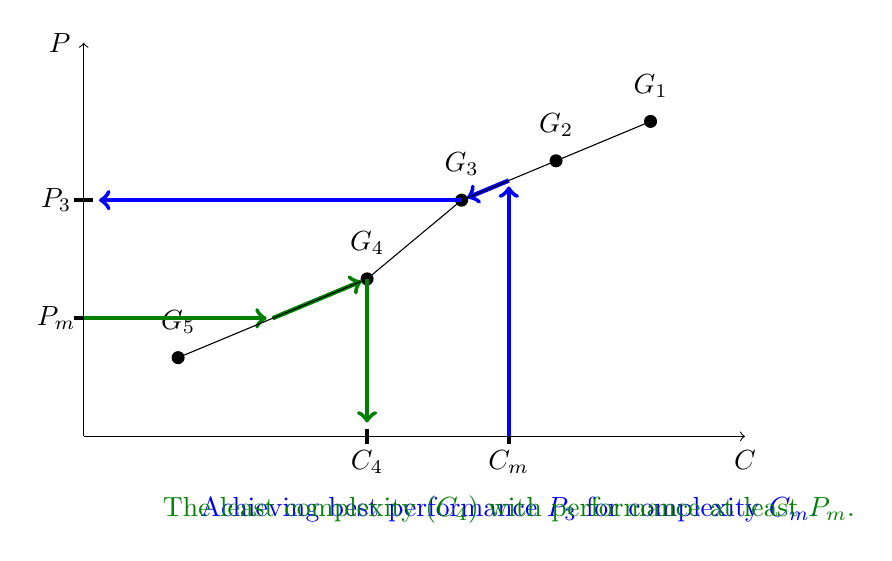
\begin{tikzpicture}[xscale=1.2]
\tikzset{point/.style={circle, fill=black, draw=black, inner sep=1pt, minimum size=1ex}}
\tikzset{b/.style={rectangle, fill=black, draw=black, inner sep=1pt, minimum size=1ex}}
\draw[->] (0,0) -- (7,0) node [pos=1, yshift=-2ex,, fill=white, inner sep=2px] {$C$};
\draw[->] (0,0) -- (0,5) node [pos=1, xshift=-2ex, fill=white, inner sep=2px] {$P$};

\node[point] at (1,1) (p1) {};
\node[above of=p1, node distance=3ex] {$G_5$};
\node[point] at (3,2) (p2) {}; \node[above of=p2, node distance=3ex] {$G_4$};
\node[point] at (4,3) (p3) {};
\node[above of=p3, node distance=3ex] {$G_3$};
\node[point] at (5,3.5) (p4) {};
\node[above of=p4, node distance=3ex] {$G_2$};
\node[point] at (6,4) (p5) {};
\node[above of=p5, node distance=3ex] {$G_1$};
\uncover<2>{
\draw[ultra thick] (4.5, 0.1) -- (4.5, -0.1) node [pos=1, yshift=-1.5ex] (CM) {$C_m$};
\draw[->, ultra thick, shorten >=0.5ex, color=blue] (4.5, 0) -- (4.5, 3.25);
\draw[->, ultra thick,shorten >=0.5ex, color=blue] (4.5, 3.25) -- (4, 3);
\draw[->, ultra thick,shorten >=0.5ex, color=blue] (4, 3) -- (0.1, 3);
\draw[ultra thick] (0.1, 3) -- (-0.1, 3) node [pos=1, xshift=-1.5ex] {$P_3$};
\node[below of=CM, node distance=4ex, color=blue] {Achieving best performance $P_3$ for complexity $C_m$.};
}
\uncover<3>{
\draw[ultra thick] (0.1, 1.5) -- (-0.1, 1.5) node [pos=1, xshift=-1.5ex] {$P_m$};
\draw[->, shorten >=0.5ex,
ultra thick,color=green!50!black] (0, 1.5) -- (2, 1.5);
\draw[->, shorten >=0.5ex, ultra thick, color=green!50!black] (2, 1.5) -- (3, 2);
\draw[->, shorten >=0.5ex,
ultra thick,color=green!50!black] (3, 2) -- (3, 0.1);
\draw[ultra thick] (3, 0.1) -- (3,-0.1) node [pos=1, yshift=-1.5ex]  {$C_4$};
\node[below of=CM, node distance=4ex, color=green!50!black] {The least complexity ($C_4$) with performance at least  $P_m$.};
}

\draw[-] (p1) -- (p2) -- (p3) -- (p4) -- (p5);
\end{tikzpicture}
